\documentclass[a4paper, 11pt]{article}
\usepackage{comment} % enables the use of multi-line comments (\ifx \fi) 
\usepackage{lipsum} %This package just generates Lorem Ipsum filler text. 
\usepackage{fullpage} % changes the margin
\usepackage{graphicx}
\usepackage{color}
\graphicspath{ {./images/} }
\usepackage[utf8]{inputenc}

\usepackage{listings}
\usepackage{xcolor}

%New colors defined below
\definecolor{codegreen}{rgb}{0,0.6,0}
\definecolor{codegray}{rgb}{0.5,0.5,0.5}
\definecolor{codepurple}{rgb}{0.58,0,0.82}
\definecolor{backcolour}{rgb}{0.95,0.95,0.92}

%Code listing style named "mystyle"
\lstdefinestyle{mystyle}{
  backgroundcolor=\color{backcolour},   commentstyle=\color{codegreen},
  keywordstyle=\color{magenta},
  numberstyle=\tiny\color{codegray},
  stringstyle=\color{codepurple},
  basicstyle=\ttfamily\footnotesize,
  breakatwhitespace=false,         
  breaklines=false,                 
  captionpos=h,                    
  keepspaces=true,                 
  numbers=left,                    
  numbersep=5pt,                  
  showspaces=false,                
  showstringspaces=false,
  showtabs=false,                  
  tabsize=2
}

%"mystyle" code listing set
\lstset{style=mystyle}

\begin{document}
%Header-Make sure you update this information!!!!

\noindent
\large\textbf{Tema de cas\u{a}} \hfill \textbf{Programarea Aplica\c{t}iilor \^{i}n Timp Real} \\
\normalsize Echipa: Necula Leonard-Gabriel | Mihăilescu Dan-Ionuț  \hfill Sem. 2, 2020-2021 \\ 
\normalsize e-mail: necula.leonard.gabriel@gmail.com | dan.mihailescu1007@stud.acs.upb.ro \\
\\
\large\textbf{\textcolor{blue}{SISTEM DE \^{I}MBUTELIERE}}



\section{Introducere - prezentarea problemei}

\hspace{2pc} \^{I}mbutelierea sticlelor ce vin pe o band\u{a} transportoare. Linia de automatizare a acestei opera\c{t}ii con\c{t}ine dou\u{a} sta\c{t}ii de lucru:
\begin{itemize}
    \item o sta\c{t}ie de umplere a sticlelor, umplerea unei sticle se face \^{i}ntr-un timp $t_{umplere}$ 
    \item o sta\c{t}ie de ad\u{a}ugare a dopului, ad\u{a}ugarea dopului se face \^{i}n timpul $t_{dop}$ 
\end{itemize}
Elemente sistem:
\begin{enumerate}
    \item motor band\u{a} transportoare
    \item senzor detec\c{t}ie sticl\u{a} goal\u{a}
    \item senzor detec\c{t}ie sticl\u{a} f\u{a}r\u{a} dop
\end{enumerate}




\subsection{Pas 1. Definire problem\u{a}}

\hspace{2pc}S\u{a} se implementeze o aplica\c{t}ie de simulare a unui proces de \^{i}mbuteliere. Aceast\u{a} aplica\c{t}ie con\c{t}ine urm\u{a}toarele taskuri:

\begin{itemize}
\item task 1 (umplere sticl\u{a} cu lichid)
\item task 2 (ad\u{a}ugare dop)
\item task 3 (pornire/oprire band\u{a} transportoare)
\end{itemize}
 
 \begin{flushleft}
Condi\c{t}iile impuse sunt urm\u{a}toarele:
\end{flushleft}

\begin{itemize}
\item banda transportoare se opre\c{s}te atunci c\^{a}nd apare o sticl\u{a} simultan \^{i}n fa\c{t}a senzorului de detec\c{t}ie sticl\u{a} goal\u{a} \c{s}i al senzorului de detec\c{t}ie sticl\u{a} f\u{a}r\u{a} dop;
\item banda transportoare reporne\c{s}te atunci c\^{a}nd taskurile de umplere c\^{a}t \c{s}i cel de ad\u{a}ugare dop \c{s}i-au terminat execu\c{t}ia;
\item procesul \^{i}ncepe cu sticle prezente \^{i}n fa\c{t}a ambelor sta\c{t}ii de lucru
\end{itemize}


\newpage 

\section{Analiza problemei}


\subsection{Exemplu: Pas 2. Analiza cerin\c{t}elor} 

Evenimente posibile:
\begin{itemize}
    \item detectarea unei sticle \^{i}n dreptul sta\c{t}iei de umplere
    \item detectarea unei sticle \^{i}n dreptul sta\c{t}iei de ad\u{a}ugare a dopului
\end{itemize}

\begin{flushleft}
Ac\c{t}iuni posibile:
\end{flushleft}
\begin{itemize}
    \item pornire/oprire band\u{a} transportoare la dete\c{t}ia sticle
    \item umplerea \c{s}i ad\u{a}ugarea dopului
\end{itemize}



\begin{flushleft}
Situa\c{t}ii imposibile:
\end{flushleft}
\begin{itemize}
\item sticlele nu vin \^{i}n acela\c{s}i timp la cele 2 sta\c{t}ii de lucru
\item banda nu se opre\c{s}te \^{i}n momentul \^{i}n care cei doi senzori detecteaz\u{a} prezen\c{t}a sticlelor la cele 2 sta\c{t}ii de lucru
\end{itemize}



\section{Definirea structurii aplica\c{t}iei}



\subsection{ Pas 3. Definirea taskurilor care compun aplica\c{t}ia}

\^{I}n cazul aplica\c{t}iei prezentate taskurile sunt:

\begin{itemize}
\item task 1 (umplere sticl\u{a} cu lichid)
\item task 2 (ad\u{a}ugare dop)
\item task 3 (pornire/oprire band\u{a} transportoare)
\end{itemize}
 


\section{Definirea solu\c{t}iei \^{i}n vederea implement\u{a}rii}

\hspace{2pc}Rezolvarea problemei propuse a fost f\u{a}cut\u{a} \^{i}n Eclipse utiliz\^{a}nd limbajul Java.
\begin{flushleft}
Mecanismele utilizate:
\end{flushleft}

\begin{itemize}
    \item excludere mutual\u{a}
    \item sincronizare pe condi\c{t}ie de timp
    \item \^{i}mp\u{a}r\c{t}irea problemei \^{i}n clase conform paradigmei OOP
\end{itemize}

\subsection{Pas 4. Solu\c{t}ie de implementare}

\hspace{2pc}Pentru problema prezentat\u{a} avem nevoie de urm\u{a}toarele mecanisme de comunicare \^{i}ntre taskuri semnafoare generalizate, mutex-uri.
Pentru vizualizarea taskurilor \c{s}i a sincronizarilor vede\c{t}i figura \^{i}n Fig.~\ref{fig:taskuri}.

\begin{itemize}
\item aleg un semafoar generalizat (e.g. \textit{counting semaphore}) $S_2$, cu valorea ini\c{t}ial\u{a}  $S_2 = 0$ \c{s}i dou\u{a} semafoare binare $S_0$, $S_1$ cu valorile ini\c{t}iale $S_0 = 0$, $S_1 = 0$.
\item folosesc un mutex pentru excluderea mutual\u{a} a accesului la zona de memorie pentru statusul benzii transportoare (\textit{nu vreau ca opera\c{t}iile de read \c{s}i write s\u{a} se poat\u{a} executa concomitent})
\end{itemize}


\begin{figure} [!htb]
\centering
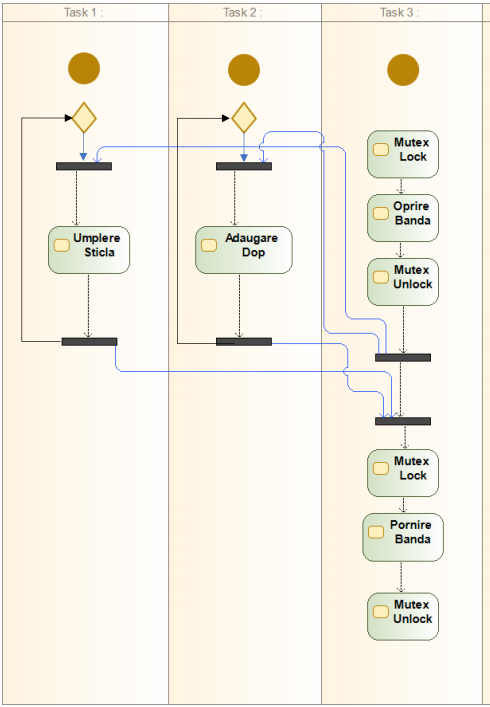
\includegraphics[width=10cm]{./images/SolutieImplementare.png}
\caption{\label{fig:taskuri}Solu\c{t}ie implementare - organigrame taskuri}
\end{figure} 

\clearpage
\section{Implementarea solu\c{t}iei}

\subsection{Cod program}

Detalii de implementare:

\begin{itemize}
\item pentru simularea prezen\c{t}ei sticlelor la \^{i}nceputul simul\u{a}rii utiliz\u{a}m un fir de execu\c{t}ie ce ruleaz\u{a} la \^{i}nceputul programului, urm\^{a}nd s\u{a} ruleze ciclic la $t_{detectare}$ secunde
\item rularea ciclic\u{a} a taskului de control al benzii transportoare din $t_{detectare}$ \^{i}n $t_{detectare}$ secunde am utilizat un timer (\textit{vezi clasa Timer}) 
\item pentru asigurarea accesului unui singur task la zona de memorie a statusului benzii transportoare folosim un mutex
\end{itemize}


Cod program:

\medskip
\medskip

\noindent

{\small
\begin{lstlisting}[language=Java, caption=Java_code]

package Implementare;

import Semafoare.SemBin;
import Semafoare.Semafor;

// Definire lista de variabile globale prin intermediul
// unei interfete

public interface GVL {
	public static Semafor S2 = new Semafor();
	public static SemBin  S0 = new SemBin();
	public static SemBin  S1 = new SemBin();
}

package Implementare;

public class TaskDop extends Thread {

	private String task_name;
	private int task_time;
	
	public TaskDop(String task_name, int task_time)
	{
		this.task_name = task_name;
		this.task_time = task_time;
	}
	
	public TaskDop()
	{
		this.task_name = "Default_Name";
		this.task_time = 1000;
	}
	
	@Override 
	public void run()
	{
		while(true)
		{
			
			GVL.S1.sem_wait();
			
			System.out.println("A inceput task-ul de " + task_name);
			
			try {
				TaskDop.sleep(task_time);
			} catch (InterruptedException e) {
				e.printStackTrace();
			}
			
			System.out.println("S-a terminat task-ul de " + task_name);
			GVL.S2.sem_post();
			
		}
	}
}

package Implementare;

public class TaskUmplere extends Thread {

	private String task_name;
	private int task_time;
	
	public TaskUmplere(String task_name, int task_time)
	{
		this.task_name = task_name;
		this.task_time = task_time;
	}
	
	public TaskUmplere()
	{
		this.task_name = "Default_Name";
		this.task_time = 1000;
	}
	
	@Override 
	public void run()
	{
		while(true)
		{
			
			GVL.S0.sem_wait();
			System.out.println("A inceput task-ul de " + task_name);
			
			try {
				TaskUmplere.sleep(task_time);
			} catch (InterruptedException e) {
				e.printStackTrace();
			}
			
			System.out.println("S-a terminat task-ul de " + task_name);
			GVL.S2.sem_post();
			
		}
	}
}

package Implementare;

import java.util.TimerTask;

public class TaskBanda extends TimerTask {
	
	int state = 0;
	static int initial = 0;
	
	public TaskBanda(int state)
	{
		this.state = state;
	}
	
	public TaskBanda()
	{
		this.state = 0;
	}
	
	@Override
	public void run() {
		
		if(initial != 0) {
			synchronized(this) {
				System.out.println("Oprire banda");
				this.state = 0; // Oprire banda
			}

		}
		else
			initial = 1;
		
		GVL.S0.sem_post();
		GVL.S1.sem_post();
		
		GVL.S2.sem_wait();
		GVL.S2.sem_wait();
		
		synchronized(this) {
			System.out.println("Repornire banda");
			this.state = 1; // Repornire banda
		}
		
		
	}
	
}



package Implementare;

import java.util.Timer;

import Semafoare.SemBin;
import Semafoare.Semafor;



public class Runner {
	
	public static void main(String[] args) {
		// TODO Auto-generated method stub
		int t_umplere = 1000 * 2;
		int t_dop = 1000 * 5;
		int t_detectare = 1000 * 15;
		
		TaskUmplere T1 = new TaskUmplere("umplere a sticlei", t_umplere);
		TaskDop T2 = new TaskDop("adaugare a dopului", t_dop);
		TaskBanda T3 = new TaskBanda();
		
		
		Timer timer_banda = new Timer();
		timer_banda.schedule(T3, 0, t_detectare);
		T1.start();
		T2.start();
		
	}

}


\end{lstlisting}
}



\section{Testarea aplica\c{t}iei si validarea solu\c{t}iei propuse}

\hspace{2pc}Pentru rularea aplica\c{t}iei deschide\c{t}i aplica\c{t}ia Eclipse, importa\c{t}i proiectul \c{s}i rula\c{t}i clasa $Runner.java$.

Mai jos ave\c{t}i un exemplu de rulare a codului \^{i}n Eclipse:


\begin{figure} [!htb]
\centering
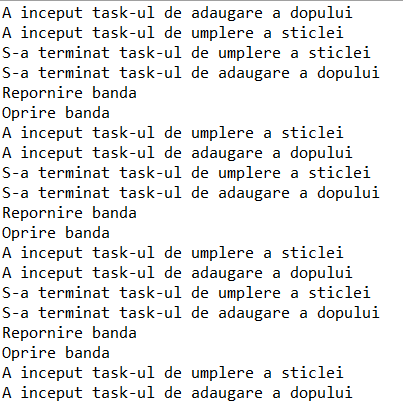
\includegraphics[width=12cm]{./images/Exemplu_rulare.png}
\caption{\label{fig:exemplu}Exemplu output}
\end{figure} 

Dup\u{a} cum pute\c{t}i observa rezultatele sunt cele a\c{s}teptate, de asemenea sunt identice cu cele din cadrul aplica\c{t}iei implementate \^{i}n C-POSIX, singura diferen\c{t}\u{a} fiind dat\u{a} de lipsa semnalelor pentru afi\c{s}are statusului benzii, aceast\u{a} afi\c{s}are fiind f\u{a}cut\u{a} acum de task-ul ce porne\c{s}te \c{s}i opre\c{s}te banda transportoare.

%\begin{thebibliography}{9}
%\bibitem{Robotics} Fred G. Martin \emph{Robotics Explorations: A Hands-On Introduction to Engineering}. New Jersey: Prentice Hall.
%
%\bibitem{Flueck}  Flueck, Alexander J. 2005. \emph{ECE 100}[online]. Chicago: Illinois Institute of Technology, Electrical and Computer Engineering Department, 2005 [cited 30
%August 2005]. Available from World Wide Web: (http://www.ece.iit.edu/~flueck/ece100).
%\end{thebibliography}

\end{document}
